\documentclass[12pt, letterpaper]{article}

\usepackage[english]{babel} % Sets the language and regional settings for English documents
\usepackage[utf8]{inputenc} % Allows the use of UTF-8 characters in the document
\usepackage[T1]{fontenc} % Specifies t\subsubsection*{Forma canónica reducida}
\usepackage[margin=2cm]{geometry} % Sets the page margins
\usepackage{makeidx} % Enables the creation of indexes
% \usepackage{natbib} % Provides flexible bibliography support
\usepackage{url} % Allows the use of URLs
\usepackage{enumitem} % Customizes the appearance of lists
\usepackage{listings} % Provides syntax highlighting for code listings
\usepackage[dvipsnames]{xcolor} % Allows the use of colors
\usepackage{parskip} % Modifies paragraph spacing
\usepackage{graphicx} % Enables the inclusion of graphics
\usepackage{tikz} % Allows the creation of graphics and diagrams
\usepackage{float}
\usepackage{hyperref} % Enables the creation of hyperlinks
\usepackage{amsmath} % Provides additional math environments and commands
\usepackage{circuitikz} % Allows the creation of electrical circuits
\usepackage{adjustbox} % Adjusts the size of the circuit diagrams
\usepackage{tcolorbox}
\usepackage{diagbox} % Allows the use of diagonal boxes in table cells
\usepackage{colortbl} % Allows coloring of table cells
\hypersetup{
    colorlinks=true,
    linkcolor=blue,
    urlcolor=blue
}
\usepackage{breakurl} % permite que los links se rompan en varias líneas
\definecolor{mygray}{gray}{0.9}

\usetikzlibrary{shapes.geometric, positioning}

\lstset{
	language=SQL,
	basicstyle=\ttfamily\small,
	keywordstyle=\color{blue},
	commentstyle=\color[rgb]{0,0.5,0},
	stringstyle=\color{red},
	numbers=left,
	numberstyle=\tiny\color{gray},
	stepnumber=1,
	numbersep=10pt,
	backgroundcolor=\color{white},
	showspaces=false,
	showstringspaces=false,
	breaklines=true,
	frame=single,
	tabsize=2, captionpos=b, lineskip=-1pt,
	extendedchars=true,
	literate={á}{{\'a}}1 {é}{{\'e}}1 {í}{{\'i}}1 {ó}{{\'o}}1 {ú}{{\'u}}1 {Á}{{\'A}}1 {É}{{\'E}}1 {Í}{{\'I}}1 {Ó}{{\'O}}1 {Ú}{{\'U}}1 {ñ}{{\~n}}1 {Ñ}{{\~N}}1 {¿}{{\textquestiondown}}1 {¡}{{\textexclamdown}}1
}

% VHDL language configuration
\lstdefinelanguage{VHDL}{
	morekeywords={entity, architecture, signal, port, in, out, inout, begin, end, process, if, then, else, elsif, case, when, others, for, while, loop, wait, library, use, std_logic, std_logic_vector, integer, boolean, rising_edge, falling_edge, component, generic, map, downto, to, and, or, not, xor, nand, nor, xnor},
	morecomment=[l]{--},
	morestring=[b]",
	sensitive=false,
	alsoletter={_}
}

% VHDL listings style
\lstdefinestyle{vhdl}{
	language=VHDL,
	basicstyle=\ttfamily\small,
	keywordstyle=\color{blue}\bfseries,
	commentstyle=\color[rgb]{0,0.6,0}\itshape,
	stringstyle=\color{red},
	numbers=left,
	numberstyle=\tiny\color{gray},
	stepnumber=1,
	numbersep=10pt,
	backgroundcolor=\color{white},
	showspaces=false,
	showstringspaces=false,
	breaklines=true,
	frame=single,
	tabsize=2,
	captionpos=b,
	lineskip=-1pt,
	extendedchars=true
}

\graphicspath{ {./img/} } % Sets the path for the graphics

\newlist{biblio}{enumerate}{1}
\setlist[biblio,1]{label=[\arabic*]}

\makeindex

\begin{document}

\begin{titlepage}

	\begin{tikzpicture}[remember picture,overlay]
		\node[anchor=north west, inner sep=30] at (current page.north west) {
			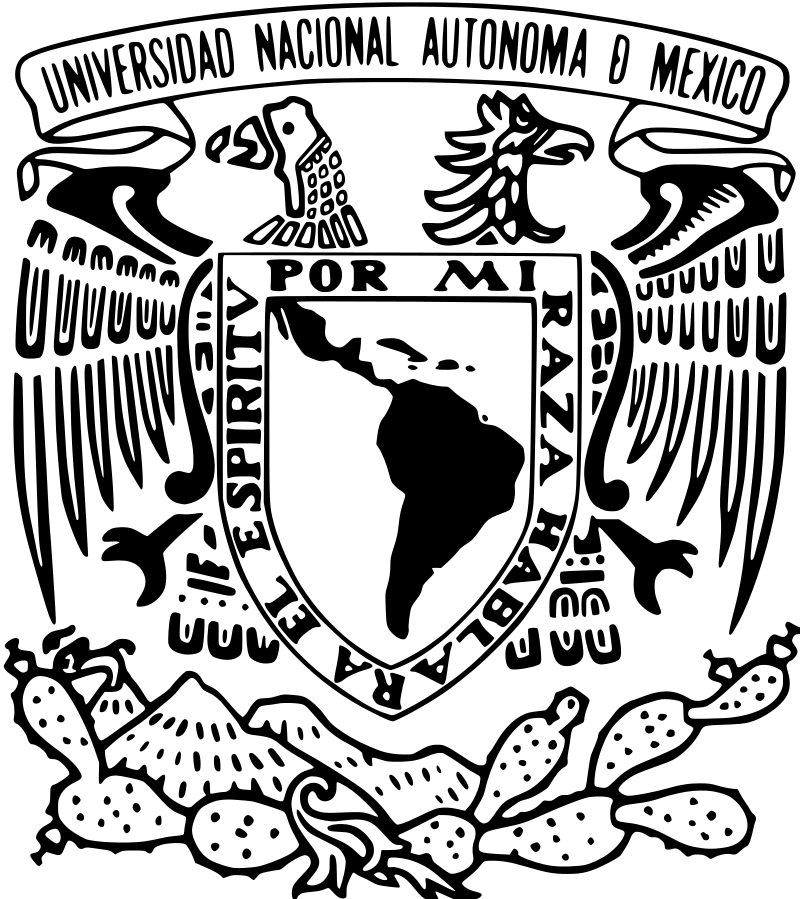
\includegraphics[width=4cm]{escudoUNAM.png}
		};

		\node[anchor=north east, inner sep=30] at (current page.north east) {
			
\includegraphics[width=4cm]{escudoFI.png}
		};
	\end{tikzpicture}

	\begin{center}
		\vspace*{3cm}

		\Huge
		\textbf{Previo 3 - Medición de Potencia en Sistemas Eléctricos}\\

		\vspace{2.5cm}

		\Huge
		\textbf{Facultad de Ingeniería}\\
		Circuitos Eléctricos\\
		\textbf{Ing. Martha Isela Torres Hernández} \\
		2026-1\\

		\vspace{2.5cm}

		%grupo de la materia
		\textbf{Grupo:} 4\\

		\vspace{2.5cm}

		\Huge
		\textbf{Integrantes Brigada 6:}\\
		Tepal Briseño Hansel Yael\\
		Ugartechea González Luis Antonio\\
		%fecha de entrega
		\textbf{Fecha de entrega:} 14 de octubre de 2025\\
		\vspace{2.5cm}
	\end{center}

\end{titlepage}

\section{Encontrar las expresiones para \(S_{3 \phi}\), \(P_{3 \phi}\) y \(Q_{3 \phi}\), para una carga equilibrada conectada en Delta.}

\begin{figure}[H]
	\centering
	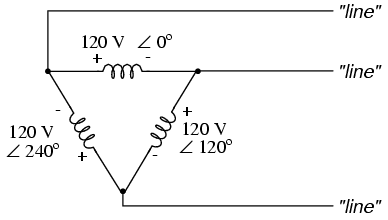
\includegraphics[width=0.5\textwidth]{circuito_delta.png}
	\caption{Carga equilibrada en conexión Delta}
\end{figure}

Para este ejercicio es necesario tener en cuenta que el voltaje de fase y el voltaje de línea en una conexión en delta son iguales, es decir:

\[V_{F} = V_{L}\]

Esto se debe a que como tal no existe el neutro. Entonces para obtener las expresiones de potencia en una conexión en delta, se utilizan las siguientes fórmulas:

\begin{tcolorbox}[colback=mygray, colframe=LimeGreen, boxrule=0.7pt, arc=2pt, boxsep=1pt, left=2pt, right=2pt, top=2pt, bottom=2pt, title=\(S_{3 \phi}\) para carga en Delta]
\[S_{3 \phi} = \sqrt{3} \cdot |V_{L}| \cdot |I_{L}|\]
\end{tcolorbox}

\begin{tcolorbox}[colback=mygray, colframe=LimeGreen, boxrule=0.7pt, arc=2pt, boxsep=1pt, left=2pt, right=2pt, top=2pt, bottom=2pt, title=\(P_{3 \phi}\) para carga en Delta]
\[P_{3 \phi} = \sqrt{3} \cdot |V_{L}| \cdot |I_{L}| \cos(\phi)\]
\end{tcolorbox}

\begin{tcolorbox}[colback=mygray, colframe=LimeGreen, boxrule=0.7pt, arc=2pt, boxsep=1pt, left=2pt, right=2pt, top=2pt, bottom=2pt, title=\(Q_{3 \phi}\) para carga en Delta]
\[Q_{3 \phi} = \sqrt{3} \cdot |V_{L}| \cdot |I_{L}| \sin(\phi)\]
\end{tcolorbox}

Para esto primero debemos de obtener la corriente de línea en función de la corriente de fase. En una conexión en delta, la relación entre la corriente de línea \(I_{L}\) y la corriente de fase \(I_{F}\) es:

\begin{tcolorbox}[colback=mygray, colframe=NavyBlue, boxrule=0.7pt, arc=2pt, boxsep=1pt, left=2pt, right=2pt, top=2pt, bottom=2pt, title=Relación entre \(I_{L}\) e \(I_{F}\) en Delta]
\[I_{L} = \sqrt{3} \cdot I_{F}\]
\end{tcolorbox}

\section{Qué expresiones tiene que usar para encontrar las potencias \(S_{3 \phi}\), \(P_{3 \phi}\) y \(Q_{3 \phi}\), para el motor trifásico de inducción conectado en Estrella mostrado en la siguiente figura.}

\begin{figure}[H]
	\centering
	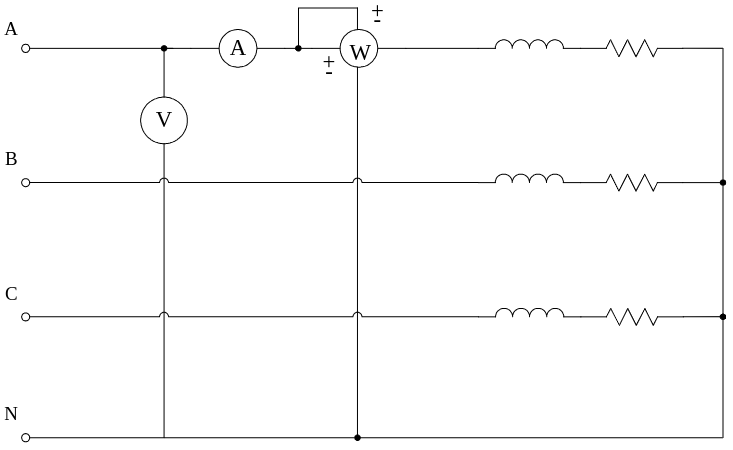
\includegraphics[width=0.7\textwidth]{motor_induccion.png}
	\caption{Motor trifásico de inducción en conexión Estrella}
\end{figure}

Para un motor trifásico de inducción conectado en estrella, las expresiones para las potencias \(S_{3 \phi}\), \(P_{3 \phi}\) y \(Q_{3 \phi}\) son las mismas que para una carga equilibrada en estrella. Estas expresiones son:

\begin{itemize}
	\item Potencia aparente:
	\(
	S_{3 \phi} = \sqrt{3} \cdot |V_{L}| \cdot |I_{L}|
	\)
	\item Potencia activa:
	\(
	P_{3 \phi} = \sqrt{3} \cdot |V_{L}| \cdot |I_{L}| \cos(\phi)
	\)
	\item Potencia reactiva:
	\(
	Q_{3 \phi} = \sqrt{3} \cdot |V_{L}| \cdot |I_{L}| \sin(\phi)
	\)
\end{itemize}

Obteniendo la potencia activa tenemos que colo existe un wattmetro que mide la potencia activa del motor, por lo que la expresión para la potencia activa es:

\[P_{3 \phi} = 3 \cdot V_{F} \cdot I_{F} \cos(\phi)\]

Para la potencia reactiva y aparente, se utilizan las mismas expresiones que para una carga equilibrada en estrella.

\begin{itemize}
	\item Potencia aparente:
	\(
	S_{3 \phi} = \sqrt{3} \cdot |V_{L}| \cdot |I_{L}|
	\)
	\item Potencia reactiva:
	\(
	Q_{3 \phi} = \sqrt{3} \cdot |V_{L}| \cdot |I_{L}| \sin(\phi)
	\)
\end{itemize}

\section{En el método de los 2 wattmetros, existe un valor del ángulo \(\phi\) para el cual, uno de los dos wattmetros marca una lectura cero; de acuerdo a la Fig. 3 encuentre el valor absoluto de \(\phi\) y compruébelo matemáticamente según las ecuaciones:}

\begin{itemize}
	\item \(P_{W1} = |V_{L}| \cdot |I_{L}| \cos \left(\phi - \frac{\pi}{6} \right) \Rightarrow P_{W1} = |V_{L}| \cdot |I_{L}| \cos \left(\phi - 30^{\circ} \right)\)
	\item \(P_{W2} = |V_{L}| \cdot |I_{L}| \cos \left(\phi + \frac{\pi}{6} \right) \Rightarrow P_{W2} = |V_{L}| \cdot |I_{L}| \cos \left(\phi + 30^{\circ} \right)\)
\end{itemize}

\begin{figure}[H]
	\centering
	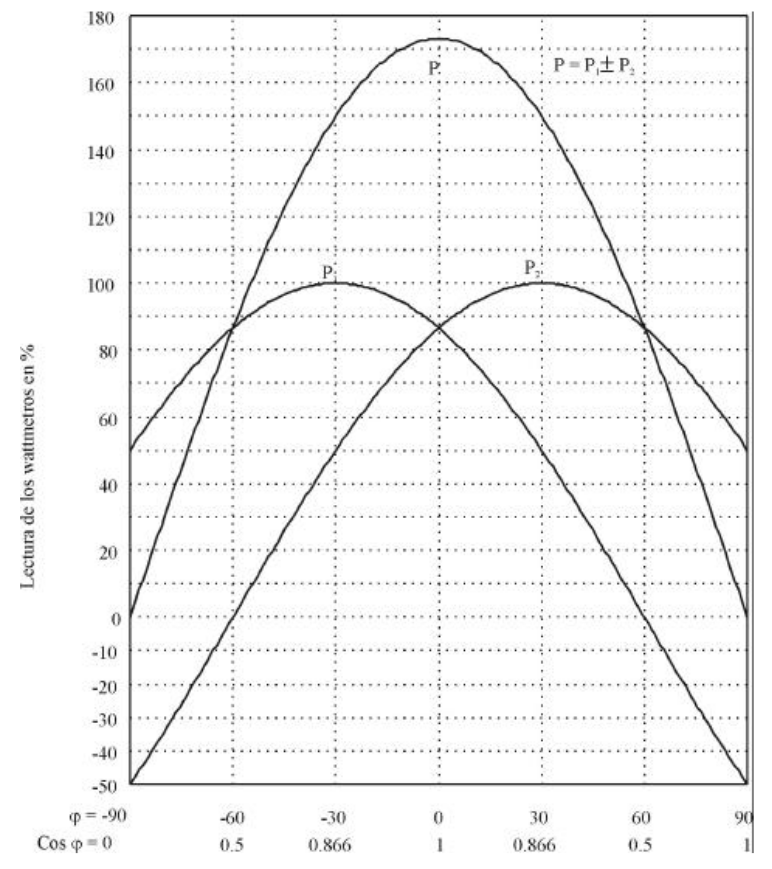
\includegraphics[width=0.8\textwidth]{figura3.png}
	\caption{Gráfica de Lecturas de \( P_{W1} \) y \( P_{W2} \) en porciento para el método de los 2 wattmetros}
\end{figure}

\newpage

Para encontrar el ángulo donde uno de los wattmetros marca una lectura cero, se puede igualar la ecuación de \(P_{W1}\) a cero y resolver para \(\phi\):

\[0 = |V_{L}| \cdot |I_{L}| \cos \left(\phi - 30^{\circ} \right)\]

De aquí se deduce que:

\[\cos \left(\phi - 30^{\circ} \right) = 0\]

Esto ocurre cuando:

\(\phi - 30^{\circ} = 90^{\circ} \Rightarrow \phi = 120^{\circ}\) o cuando: \(\phi - 30^{\circ} = -90^{\circ} \Rightarrow \phi = -60^{\circ}\)

Por lo tanto, los valores de \(\phi\) donde uno de los wattmetros marca cero son:

\begin{tcolorbox}[colback=mygray, colframe=ForestGreen, boxrule=0.7pt, arc=2pt, boxsep=1pt, left=2pt, right=2pt, top=2pt, bottom=2pt, title=Valores de \(\phi\)]
\begin{center}
	\( \phi = 120^{\circ}\) o \( \phi = -60^{\circ}\)
\end{center}
\end{tcolorbox}

\section{¿Identifique los wattmetros \(W_1\) y \(W_2\) en el diagrama de la Fig. 4? Considere que la carga es inductiva y resistiva balanceada.}

\begin{figure}[H]
	\centering
	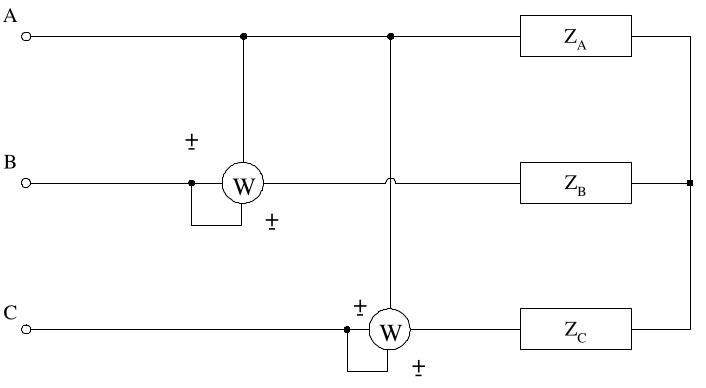
\includegraphics[width=0.6\textwidth]{figura4.png}
	\caption{Lectura de la potencia activa por el método de los dos wattmetros}
\end{figure}

El primer wattmetro \(W_1\) está conectado en la línea B, midiendo la potencia activa en esa fase. El segundo wattmetro \(W_2\) está conectado entre la línea C y la línea B, midiendo la potencia activa en esa fase. Esto nos deja las siguientes expresiones para cada wattmetro:

\begin{itemize}
	\item Para el wattmetro \(W_1\):
	\(
	P_{W1} = |V_{B-A}| \cdot |I_{B}| \cos \left(\phi \right)
	\)
	\item Para el wattmetro \(W_2\):
	\(
	P_{W2} = |V_{C-A}| \cdot |I_{C}| \cos \left(\phi \right)
	\)
\end{itemize}

\section{En una carga trifásica balanceada, se obtuvieron los valores que se dan a continuación. Considerando el diagrama de conexiones de la Fig. 5, determine el tipo de carga y su factor de potencia correspondiente.}

\begin{figure}[H]
	\centering
	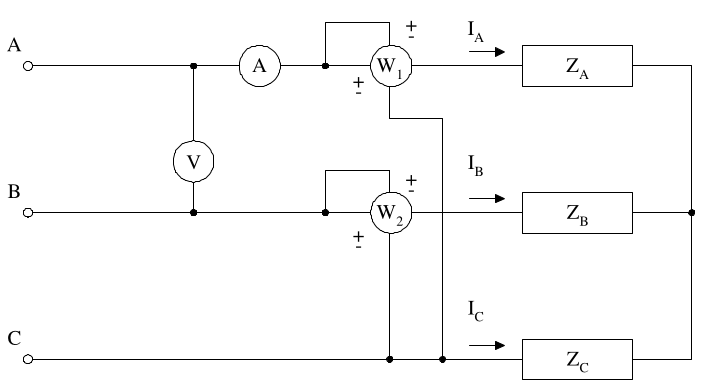
\includegraphics[width=0.7\textwidth]{figura5.png}
	\caption{Método de los dos wattmetros para medir potencia en un sistema trifásico}
\end{figure}

Con los siguientes datos:
\begin{itemize}
	\item \(V_{a-c} = 220 [\text{V}]\)
	\item \(I_{A} = 5 [\text{A}]\)
	\item \(P_{W1} = 1100 [\text{W}]\)
	\item \(P_{W2} = 550 [\text{W}]\)
\end{itemize}

Con los datos podemos obtener \(S_{3 \phi}\):

\[S_{3 \phi} = \sqrt{3} \cdot |V_{a-c}| \cdot |I_{A}| = \sqrt{3} \cdot 220 [\text{V}] \cdot 5 [\text{A}] = 1905.25 [\text{W}]\]

Ahora necesitamos obtener \(P_{3 \phi}\):

\[P_{3 \phi} = P_{W1} + P_{W2} = 1100 [\text{W}] + 550 [\text{W}] = 1650 [\text{W}]\]

Con estos valores podemos obtener el factor de potencia:

\[\text{FP} = \frac{P_{3 \phi}}{S_{3 \phi}} = \frac{1650 [\text{W}]}{1905.25 [\text{W}]} = 0.866\]

\begin{tcolorbox}[colback=mygray, colframe=ForestGreen, boxrule=0.7pt, arc=2pt, boxsep=1pt, left=2pt, right=2pt, top=2pt, bottom=2pt, title=Tipo de carga y factor de potencia]
\[FP = 0.866\]
\end{tcolorbox}

\section{Demuestre la validez de la siguiente expresión}

\[Q_{3 \phi} = \sqrt{3} (P_{W1} - P_{W2})\]

Dondde \(Q_{3 \phi}\) es la potencia reactiva trifásica, y \(P_{W1}\) y \(P_{W2}\) son los valores indicadodos por wattmetros 1 y 2 respectivamente de la figura 6.

\begin{figure}[H]
	\centering
	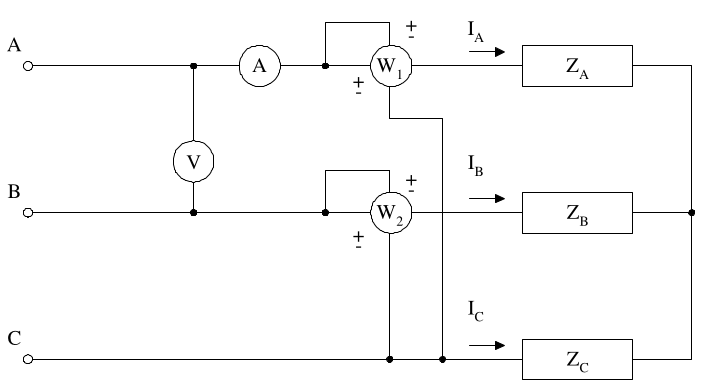
\includegraphics[width=0.6\textwidth]{figura5.png}
	\caption{Método de los dos wattmetros para medir potencia en un sistema trifásico}
\end{figure}

Tenemos para los valores de Potencia de los wattmetros:

\begin{itemize}
	\item \(P_{W1} = |V_{L}| \cdot |I_{L}| \cos \left(\phi - \frac{\pi}{6} \right) \Rightarrow P_{W1} = |V_{L}| \cdot |I_{L}| \cos \left(\phi - 30^{\circ} \right)\)
	\item \(P_{W2} = |V_{L}| \cdot |I_{L}| \cos \left(\phi + \frac{\pi}{6} \right) \Rightarrow P_{W2} = |V_{L}| \cdot |I_{L}| \cos \left(\phi + 30^{\circ} \right)\)
\end{itemize}

Utilizamos la identidad trigonométrica para la suma y resta de ángulos:

\begin{itemize}
	\item \(\cos(A - B) = \cos(A)\cos(B) + \sin(A)\sin(B)\)
	\item \(\cos(A + B) = \cos(A)\cos(B) - \sin(A)\sin(B)\)
\end{itemize}

Aplicando estas identidades a las expresiones de \(P_{W1}\) y \(P_{W2}\):

\begin{itemize}
	\item \(P_{W1} = |V_{L}| \cdot |I_{L}| \left( \cos(\phi) \cos(30^{\circ}) + \sin(\phi) \sin(30^{\circ}) \right)\)
	\item \(P_{W2} = |V_{L}| \cdot |I_{L}| \left( \cos(\phi) \cos(30^{\circ}) - \sin(\phi) \sin(30^{\circ}) \right)\)
\end{itemize}

Sustituyendo en la expresión objetivo tenemos:

\(Q_{3 \phi} = \sqrt{3} \left( |V_{L}||I_{L}| \left( \cos(\phi) \cos(30^{\circ}) + \sin(\phi) \sin(30^{\circ}) - \cos(\phi) \cos(30^{\circ}) + \sin(\phi) \sin(30^{\circ}) \right) \right)\)

Desarrollando la expresión:

\(Q_{3 \phi} = \sqrt{3} \left( |V_{L}||I_{L}| \left( 2 \sin(\phi) \sin(30^{\circ}) \right) \right)\)

\(Q_{3 \phi} = \sqrt{3} \cdot |V_{L}| \cdot |I_{L}| \cdot 2 \sin(\phi) \cdot \frac{1}{2}\)

Llegando a la expresión final:

\begin{tcolorbox}[colback=mygray, colframe=ForestGreen, boxrule=0.7pt, arc=2pt, boxsep=1pt, left=2pt, right=2pt, top=2pt, bottom=2pt, title=Expresión demostrada]
\[Q_{3 \phi} = \sqrt{3} \cdot |V_{L}| \cdot |I_{L}| \cdot \sin(\phi)\]
\end{tcolorbox}

\section{Triángulo de Potencia}

El triángulo de potencia es una herramienta gráfica fundamental en el análisis de circuitos de corriente alterna (CA). Es un triángulo rectángulo que representa visualmente la relación vectorial entre los tres tipos de potencia: Potencia Activa (P), Potencia Reactiva (Q) y Potencia Aparente (S).

\begin{figure}[H]
	\centering
	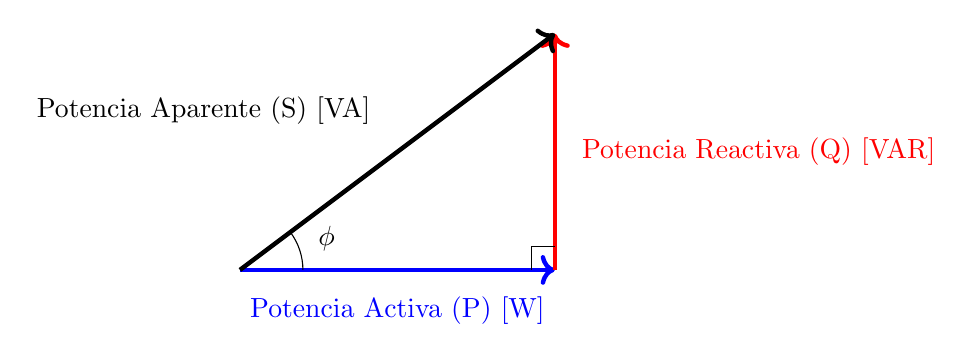
\begin{tikzpicture}

		\draw[->, ultra thick, blue] (0,0) -- (4,0) node[midway, below, yshift=-2mm] {Potencia Activa (P) [W]};
		\draw[->, ultra thick, red] (4,0) -- (4,3) node[midway, right, xshift=2mm] {Potencia Reactiva (Q) [VAR]};
		\draw[->, ultra thick, black] (0,0) -- (4,3) node[midway, above left, xshift=-2mm, yshift=2mm] {Potencia Aparente (S) [VA]};

		\draw (0.8,0) arc (0:36.87:0.8); % 36.87 grados es aprox. atan(3/4)
		\node at (1.1, 0.4) {$\phi$};

		\draw (4, 0.3) -- (3.7, 0.3) -- (3.7, 0);
	\end{tikzpicture}
	\caption{Representación del Triángulo de Potencia.}
\end{figure}

La relación matemática entre estas potencias se deriva directamente del teorema de Pitágoras:
\[ S^2 = P^2 + Q^2 \]
Donde la magnitud de la potencia aparente es:
\[ |S| = \sqrt{P^2 + Q^2} \]

\subsection*{Componentes del Triángulo}

El triángulo está compuesto por tres lados, cada uno representando un tipo de potencia:


\subsubsection*{Potencia Activa (P)}

Es el cateto adyacente al ángulo $\phi$. Representa la potencia "real" o "útil" que se consume en el circuito y se transforma en trabajo, como calor, luz o movimiento mecánico.

\begin{itemize}
	\item \textbf{Unidad:} Watts (W).
	\item \textbf{Fórmula:} \( P = |S| \cos(\phi) = |V| \cdot |I| \cos(\phi) \).
\end{itemize}

\subsubsection*{Potencia Reactiva (Q)}

Es el cateto opuesto al ángulo $\phi$. Es la potencia que no realiza un trabajo útil, pero es indispensable para el funcionamiento de componentes que almacenan energía en campos magnéticos (inductores) o eléctricos (capacitores). Esta potencia "fluye" de ida y vuelta entre la fuente y la carga.

\begin{itemize}
	\item \textbf{Unidad:} Volt-Amperes Reactivos (VAR).
	\item \textbf{Fórmula:} \( Q = |S| \sin(\phi) = |V| \cdot |I| \sin(\phi) \).
\end{itemize}

\subsubsection*{Potencia Aparente (S):}

Es la hipotenusa del triángulo. Representa la potencia total que la compañía eléctrica debe suministrar al circuito. Es la suma vectorial de la potencia activa y reactiva.

\begin{itemize}
	\item \textbf{Unidad:} Volt-Amperes (VA).
	\item \textbf{Fórmula:} \( |S| = |V| \cdot |I| \).
\end{itemize}

\subsection*{Factor de Potencia Ideal}

El \textbf{Factor de Potencia (FP)} es la relación entre la potencia activa (P) que realiza trabajo útil y la potencia aparente (S) total suministrada. En el triángulo, es el coseno del ángulo $\phi$:
\[ \text{FP} = \frac{P}{S} = \cos(\phi) \]

El \textbf{factor de potencia ideal es 1}.

Esto se logra cuando el ángulo $\phi = 0^\circ$. En esta situación ideal:
\begin{itemize}
	\item La potencia reactiva (Q) es cero.
	\item La potencia aparente es igual a la potencia activa ($S = P$).
	\item Toda la energía suministrada por la fuente se convierte en trabajo útil.
\end{itemize}

Las compañías eléctricas penalizan a las industrias con un bajo factor de potencia (muy inductivo, $\phi$ grande) porque esto significa que deben suministrar una gran cantidad de corriente (para generar S) para obtener una cantidad de trabajo útil (P) relativamente pequeña, lo que aumenta las pérdidas en las líneas de transmisión.


% \section{Bibliografía}
% \renewcommand{\refname}{}
% \begin{thebibliography}{9}
%    \bibitem{} Dr. E. García, \textit{"Diseño Digital VLSI Repaso DDM"}, presentado en el curso de Diseño Digital VLSI, Ciudad de México, 2025.
% \end{thebibliography}

\end{document}
